\documentclass[a4paper,10pt,ngerman]{scrartcl}
\usepackage{babel}
\usepackage[T1]{fontenc}
\usepackage[utf8x]{inputenc}
\usepackage[a4paper,margin=2.5cm,footskip=0.5cm]{geometry}
\usepackage{listings}

\newcommand{\Aufgabe}{Aufgabe 4: Krocket}
\newcommand{\TeamId}{00178}
\newcommand{\TeamName}{Team-Name}
\newcommand{\Namen}{Matthew Greiner}
 
% Kopf- und Fußzeilen
\usepackage{scrlayer-scrpage, lastpage}
\setkomafont{pageheadfoot}{\large\textrm}
\lohead{\Aufgabe}
\rohead{Team-ID: \TeamId}
\cfoot*{\thepage{}/\pageref{LastPage}}

\lstset{ %
  language=Java,
  basicstyle=\ttfamily\small,
  keywordstyle=\color{blue},
  commentstyle=\color{green!50!black},
  stringstyle=\color{orange},
  numbers=left,
  numberstyle=\tiny\color{gray},
  stepnumber=1,
  numbersep=5pt,
  backgroundcolor=\color{white},
  showspaces=false,
  showstringspaces=false,
  tabsize=2,
  breaklines=true,
  breakatwhitespace=true,
  frame=single,
  captionpos=b,
}

% Position des Titels
\usepackage{titling}
\setlength{\droptitle}{-1.0cm}

% Für mathematische Befehle und Symbole
\usepackage{amsmath}
\usepackage{amssymb}
\usepackage{amsthm}

% Für Bilder
\usepackage{graphicx}
\graphicspath{ {./bilder/} }

% Für Algorithmen
\usepackage{algpseudocode}

% Für Quelltext
\usepackage{listings}
\usepackage{color}
\definecolor{mygreen}{rgb}{0,0.6,0}
\definecolor{mygray}{rgb}{0.5,0.5,0.5}
\definecolor{mymauve}{rgb}{0.58,0,0.82}
\lstset{
  keywordstyle=\color{blue},commentstyle=\color{mygreen},
  stringstyle=\color{mymauve},rulecolor=\color{black},
  basicstyle=\footnotesize\ttfamily,numberstyle=\tiny\color{mygray},
  captionpos=b, % sets the caption-position to bottom
  keepspaces=true, % keeps spaces in text
  numbers=left, numbersep=5pt, showspaces=false,showstringspaces=true,
  showtabs=false, stepnumber=2, tabsize=2, title=\lstname
}
\lstdefinelanguage{JavaScript}{ % JavaScript ist als einzige Sprache noch nicht vordefiniert
  keywords={break, case, catch, continue, debugger, default, delete, do, else, finally, for, function, if, in, instanceof, new, return, switch, this, throw, try, typeof, var, void, while, with},
  morecomment=[l]{//},
  morecomment=[s]{/*}{*/},
  morestring=[b]',
  morestring=[b]",
  sensitive=true
}

% Diese beiden Pakete müssen zuletzt geladen werden
%\usepackage{hyperref} % Anklickbare Links im Dokument
\usepackage{cleveref}

% Daten für die Titelseite
\title{\textbf{\Huge\Aufgabe}}
\author{\LARGE Team-ID: \LARGE \TeamId \\\\
	    \LARGE Team-Name: \LARGE \TeamName \\\\
	    \LARGE Bearbeiter/-innen dieser Aufgabe: \\ 
	    \LARGE \Namen\\\\}
\date{\LARGE\today}

\begin{document}

\maketitle
\tableofcontents

\vspace{0.5cm}

\section{Lösungsidee / Ansatz}
\subsection{Annahme: Radius = 0}
Um diese Aufgabe zu lösen, kann der Garten als zweidimensionales Koordinatensystem interpretiert werden. Die Krockettore sind dabei Strecken, die mit einem Start- und Endpunkt mit x- und y-Koordinaten dargestellt werden.
Um herauszufinden, ob es möglich ist mit nur einem Schlag alle Tore in der Richtigen Reihenfolge zu durchqueren, muss man schauen, ob es eine Gerade gibt, die alle gegebenen Tore bzw. Strecken schneidet.
Wenn eine solche Gerade existert, dann entspricht diese der Bahn, die der Ball rollen müste, um alle Tore zu durchqueren. Der Startpunkt des Balls muss also auf dieser Gerade liegen (z.B. der Schnittpunkt von der Gerade mit dem ersten Tor), und die Schlagrichtung entspricht 
der Steigung der Gerade. 
\newline
Um zu schauen, ob so eine Gerade existert, reicht es, nur Geraden anzuschauen, die durch einen Punkt des ersten Tors und einen Punkt des zweiten Tors verlaufen. Wenn keine dieser Geraden alle Tore in schneidet, ist es unmöglich, die Aufgabe mit einem einzigen Schlag zu lösen.
Jede Gerade kann eindeutig durch zwei Punkte definiert werden: einen Punkt auf dem ersten Tor und einen Punkt auf dem zweiten Tor. Deswegen werden die Geraden gebildet, indem alle möglichen Punktkombinationen zwischen diesen beiden Toren geprüft werden.
\newline
Dann wird für jede dieser Geraden überprüft, ob sie alle Tore schneidet, wenn nein, wird die nächste Gerade überprüft, und wenn es keine Gerade gibt, gibt es keine Lösung für diese Aufgabe. Wenn eine Gerade gefunden wird, die alle Tore schneidet,
ist diese Gerade der Weg des Balls und Startpunkt und Schlagrichtung können direkt abgeleitet werden.
\subsection{Annahme: Radius $\neq$ 0}
Wenn der Radius $\neq$ 0 ist, dann ist der Ansatz mit den Geraden aufstellen gleich. Nur muss hier die Überprüfung, ob eine Gerade ein Tor schneidet, verändert werden. Denn wenn der Ball einen Radius hat, würde der Ball bei einigen Stellen nicht durch das Tor passen, auch wenn die 
aufgestellte Gerade das Tor schneidet. Um dieses Problem zu lösen, können Kreisgleichungen aufgestellt werden, die ihren Mittelpunkt bei dem Start und Endpunkt eines Tores, und den Radius von dem Ball haben. Wenn die zu überprüfende Gerade das Tor schneidet, und die beiden Kreise 
um die Pfosten des Tores nicht schneidet, dann passt der Ball durch das Tor. Wenn aber die Gerade das Tor schneidet, und auch mindestens einen der Kreise schneidet und/oder berührt, dann prallt der Ball an einem Posten ab und durchquert das Tor nicht. Somit kann diese Gerade als Lösung 
ausgeschlossen werden.
\newline

Ein simples Python Skript mit Matplotlib kann verwendet werden, um die Tore und die Lösungsgerade in einem Koordinatensystem darzustellen.

\section{Umsetzung}

\subsection{Einlesung der Daten}
Um die Daten aus einer Datei zu lesen, wird der Inhalt der Datei als ein String gespeichert, an den newline Zeichen ("\textbackslash n") gespalten und jede Zeile als ein Element in einem String Array gespeichert. Jedes Element wird an den Leerzeichen gespalten, um an die Zahlenwerte zu kommen, die als Attribute in einem 
Gate Objekt gespeichert werden. Ein Gate Objekt hat jeweils einen Start und Endpunkt als Attribute. Punkte sind Objekte mit einer x und y-Koordinate. 

\subsection{Finden einer Gerade}
Um nun eine Gerade zu finden, die alle eingelesenen Tore schneidet, kann man iterativ arbeiten und über alle möglichen Geraden iteriert wird und geprüft wird, ob sie eine Lösung des Problems ist. Dies kann man mit drei verschachelten for-Schleifen gemacht werden.
Ich gehe wie folgt vor:
\begin{itemize}
  \item [1.] Schrittweise über alle möglichen Startpunkte entlang des ersten Tors iterierieren (erste for-Schleife). Die Positionen auf dem ersten Tor sind in bestimmten Abständen (als Bruchteile der Länge des Tors) plaziert.
  \item [2.] Für jeden dieser Punkte wird über alle möglichen Punkte (hier genannt Richtungspunkte) entlang des zweiten Tors iteriert (zweite for-Schleife), welche ebenfalls mit einem Abstand, das ein Bruchteil der Länge des Tors ist, entfernt sind.
  \item [3.] Nun wird für jede Kombination aus Startpunkt und Richtungspunkt eine Gerade erstellt und überprüft, ob diese Gerade alle Tore schneidet. Es wird über alle Tore iteriert (dritte for-Schleife) und überprüft, ob \textbf{ein bestimmtes Tor geschnitten} wird oder nicht.
  Wenn das Tor geschnitten wird, wird mit dem nächsten Tor weitergemacht. Wenn nicht, dann wird aus dieser Schleife (dritte for-Schleife) gesprungen und mit dem nächsten Paar aus Start- und Richtungspunkt weitergemacht.
  \newline
  \subsubsection{Schnittpunktüberprüfung - Gerade mit einer Strecke}

  Um zu Überprüfen, ob eine Strecke und eine Gerade sich schneidet, kann so vorgegangen werden: Wenn die Gerade und Strecke parallel ist, dann gibt es keinen Schnittpunkt. Wenn sie nicht parallel sind, und die Strecke als Gerade angesehen wird, existert ein Schnittpunkt.
  Daher muss nur überprüft werden, ob dieser Schnittpunkt innerhalb den Begrenzungen der Strecke (Pfosten des Tors) liegt.
  \newline 

  Eine Gerade die durch den Punkt $(x_{1}, y_{1})$ verläuft, und den Richtungsvektor $(dx, dy)$ hat, kann in Parameterform mit Parameter $t$ wie folgt dargestellt werden ($x$ und $y$ separat dargestellt, anstatt als Vektor):
  \begin{align}
    x&=x_{1} + t \cdot dx \\
    y&=y_{1} + t \cdot dy
  \end{align}
    
  In der Parameterdarstellung sieht die Strecke mit Startpunkt $(x_{3}, y_{3})$ und Endpunkt $(x_{4}, y_{4})$ und $u$ als Linearfaktor so aus:
  \begin{align}
    x&=x_{3} + u \cdot (x_{4} - x_{3}) \quad; 0 \leq u \leq 1 \\
    y&=y_{3} + u \cdot (y_{4} - y_{3}) \quad; 0 \leq u \leq 1
  \end{align}

  Um nun die Schnittpunkte der Strecke und Gerade zu bekommen, werden die Gleichungen gleichgesetzt, wodurch sich ein Lineares Gleichungssystem bildet:

  \begin{align*}
    x_{1}+t\cdot dx&=x_{3}+u \cdot (x_{4} - x_{3}) \\
    y_{1}+t \cdot dy&=y_{3}+u\cdot (y_{4} - y_{3}) \\
  \end{align*}

  Durch umstellen, dass $t$ und $u$ auf der linken Seite sind und umformen in eine Matrixform ergibt sich die Matrix $M$:
  \begin{align}
    M = 
    \begin{pmatrix}
      dx & -(x_{4} - x_{3})\\
      dy & -(y_{4} - y_{3})
    \end{pmatrix}
    \cdot
    \begin{pmatrix}
      t \\
      u
    \end{pmatrix}
    =
    \begin{pmatrix}
      x_{3} - x_{1} \\
      y_{3} - y_{1}
    \end{pmatrix}
  \end{align}

  Daraus ergibt sich die Determinante der 2x2 Matrix als:
  \begin{align*}
    det(M) = dx \cdot (y_{4} - y_{3}) - dy \cdot (x_{4} - x_{3})
  \end{align*}

  Wenn $det(M) = 0$, dann ist die Gerade und die Strecke parallel  oder kollinear zueinander (da die Richtungsvektoren linear abhängig sind). Somit kann es \textbf{keinen Schnittpunkt} geben.
  \newline
  Andernfalls, müssen $t$ (wo auf der Gerade der Schnittpunkt ist) und $u$ (zeigt ob der Schnittpunkt auf der Strecke liegt; liegt auf der Strecke falls: $0 \leq u \leq 1$) berechnet werden.
  \newline
  Um die Parameter zu berechnen kann man mit dem Gauß-Verfahren vorgehen oder (wie ich jetzt) mit der Cramerschen Regel für 2x2 Matrixen:
  \newline
  \newline
  Somit ergibt sich $t$ aus:
  \begin{align*}
    t = 
    \frac{
      det(
        \begin{pmatrix}
          (x_{3} - x_{1}) & -(x_{4} - x_{3})\\
          (y_{3} - y_{1}) & -(y_{4} - y_{3})
        \end{pmatrix}
      )
    }{
      det(M)
    }
    = \frac{(x_{3}- x_{1}) \cdot (y_{4}- y_{3}) - (y_{3} - y_{1}) \cdot (x_{4} - x_{3})}{det(M)}
  \end{align*}

  Analog dazu ergibt sich $u$ folgendermaßen:
  \begin{align*}
    u = \frac{(x_{3}- x_{1}) \cdot dy - (y_{3} - y_{1}) \cdot dx}{det(M)}
  \end{align*}

  Falls $0 \leq u \leq 1$, dann befindet sich der Schnittpunkt auf der Strecke. Falls das nicht der Fall ist, dann liegt er nicht auf der Strecke und ist für uns unrelevant.

  \textbf{Unter der Annahme, dass der Ballradius null ist,} genügt es an dieser Stelle zu sagen, dass das Tor von dem Ball durchquert wird und es kann mit dem nächsten Tor weitergemacht werden.
  \newline
  \newline 
  \textbf{Wenn der Ballradius aber ungleich null ist,} muss überprüft werden, ob die Gerade die Kreise $(r_{Kreis} = r_{Ball})$ um die Posten schneidet (Siehe \textbf{1.2}).

  \subsubsection{Schnittpunktüberprüfung - Gerade mit einem Kreis}

  Ein Kreis mit dem Mittelpunkt $(c_{x}, c_{y})$ und dem Radius $r$ wird mathematisch so beschrieben:

  \begin{align}
  (x - c_{x})^{2} + (y - c_{y})^{2}=r^{2}
  \end{align}

  Um die Schnittpunkte von einem Kreis und einer Gerade zu berechnen, muss die parametrische Form der Geradengleichung (1)/(2) in die Kreisgleichung (6) eingesetzt werden:

  \begin{align*}
  ((x_{1} + t \cdot dx) - c_{x})^{2} + ((y_{1} + t \cdot dy) - c_{y})^{2}=r^{2}
  \end{align*}

  Nachdem man das vereinfacht und ausmultipliziert, hat man eine quadratische Gleichung in $t$:
  \begin{align*}
    a \cdot t^{2}+b \cdot t + c= 0
  \end{align*}
  mit 
  \begin{align*}
    a &= dx^{2} + dy^{2} \\
    b &= 2 \cdot (dx \cdot (x_{1} - c_{x}) + dy \cdot (y_{1} - c_{y})) \\
    c &= (x_{1} - c_{x}) ^{2} + (y_{1} - c_{y})^{2} - r^{2}
  \end{align*}

  die mit der quadratischen Lösungsformel berechnet werden kann: 
  \begin{align*}
    t = \frac{-b \pm \sqrt{\text{Diskriminante}}}{2a}
  \end{align*} 

  Falls hierbei die \textbf{Diskriminante < 0} ist, schneidet die Gerade den Kreis nicht (für diese Aufgabe bedeutet das, dass der Ball das Tor durchqueren kann). 
  \newline
  Wenn die Diskriminante = 0 ist, berührt die Gerade den Kreis und wenn sie > 0 ist, 
  gibt es zwei Schnittpunkte von der Gerade und dem Kreis. In den letzteren zwei Fällen durchquert der Ball das Tor nicht, sondern prallt an einem Posten ab.
  \newline
  Die Diskriminante berechnet sich wie folgt:
  \begin{align*}
    \text{Diskriminante} = b^{2} - 4ac
  \end{align*}



  \item [4.] Wenn eine Gerade gefunden wurde, die alle Tore schneidet, wird sie als Resultat zurückgegeben. Der Startpunkt des Schlags von Laura ist der Schnittpunkt der Geraden mit dem ersten Tor und die Richtung des Schlags entspricht der Steigung der Gerade. Da aber eine Gerade, die parallel zur y-Achse ist, nicht existert und somit die Steigung davon nicht definiert wird,
  wird als Richtung des Schlags der normierte Richtungsvektor der Gerade ausgegeben.
\end{itemize}

\section{Beispiele}
\subsection{Beispiele der BwInf-Webseite}
Hier die Ausgaben des Programmes zu den Beispielen auf der BwInf-Webseite: Zusätzlich wird das Ergebnis mit dem beigelegem python-skript und matplotlib visuell dargestellt. (Falls es ein Ergebnis gibt) Hierbei ist die
Rote Linie die Strecke des Balls von Laura, die alle Tore durchquert.
\begin{itemize}
  \item [1.] \textbf{krocket1.txt}
    \newline
    Es ist möglich mit einem Schlag alle Tore zu durchqueren.
    \newline
    Der Schlag kann als Halbgerade mit dem Startpunkt: (11.280000000000001|9.119999999999994), die durch den Punkt (17.18|12.009999999999994) verläuft, beschrieben werden.
    \newline
    Normierter Richtungsvektor: (0.8980504366047625, 0.43989250199792623), bzw. Steigung der Halbgeraden: 0.4898305084745765
    \newline
    \newline
    Darstellung (python-skript)
    \newline
    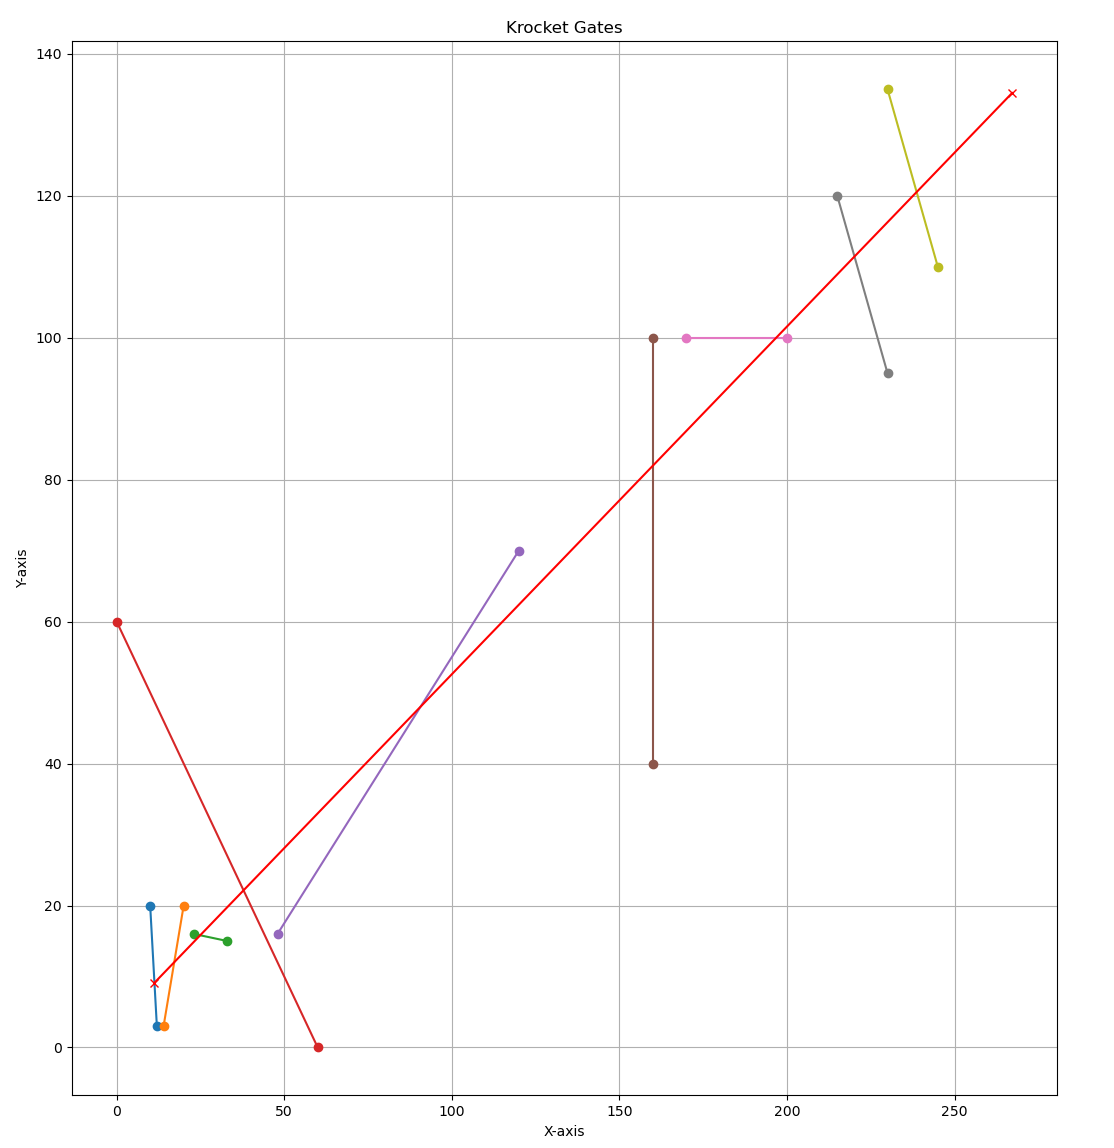
\includegraphics[scale=0.27]{krocket1.png}

  \item [2.] \textbf{krocket2.txt}
    \newline
    Es ist nicht möglich, alle Tore in der richtigen Reihenfolge mit nur einem Schlag zu durchqueren.

    Darstellung (python-skript)
    \newline
    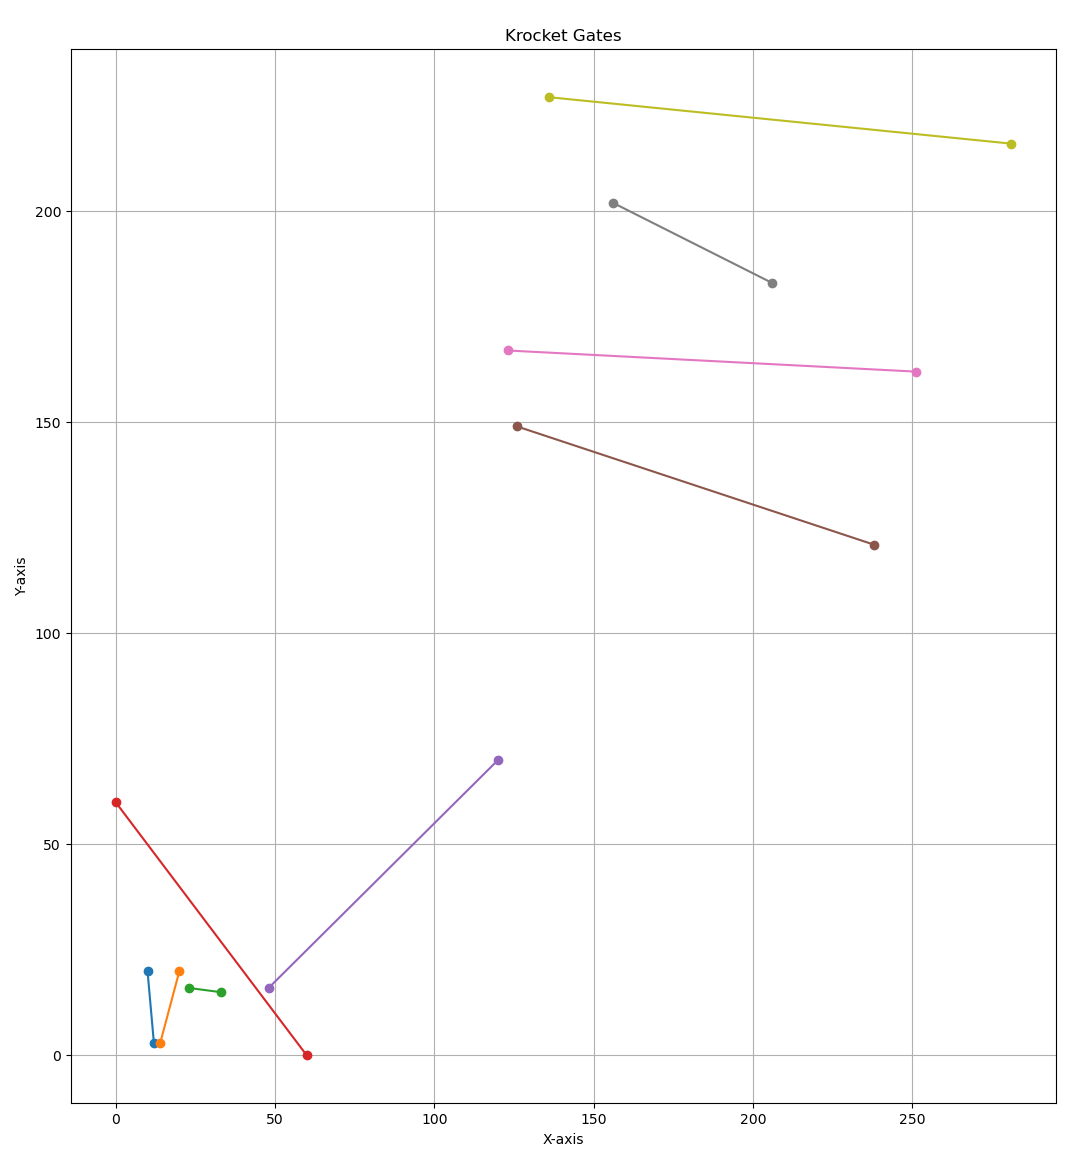
\includegraphics[scale=0.27]{krocket2.png}

  \newpage

  \item [3.] \textbf{krocket3.txt}
  \newline
  Es ist möglich mit einem Schlag alle Tore zu durchqueren.
  \newline
  Der Schlag kann als Halbgerade mit dem Startpunkt: (22.8|128.8), die durch den \newline Punkt (31628.4|125.60000000000002) verläuft, beschrieben werden.
  \newline
  Normierter Richtungsvektor: (0.9999999948744334, -1.0124787960355681E-4), bzw. Steigung der Halbgeraden: -1.0124788012250957E-4
  \newline
  \newline
  Darstellung (python-skript)
  \newline
  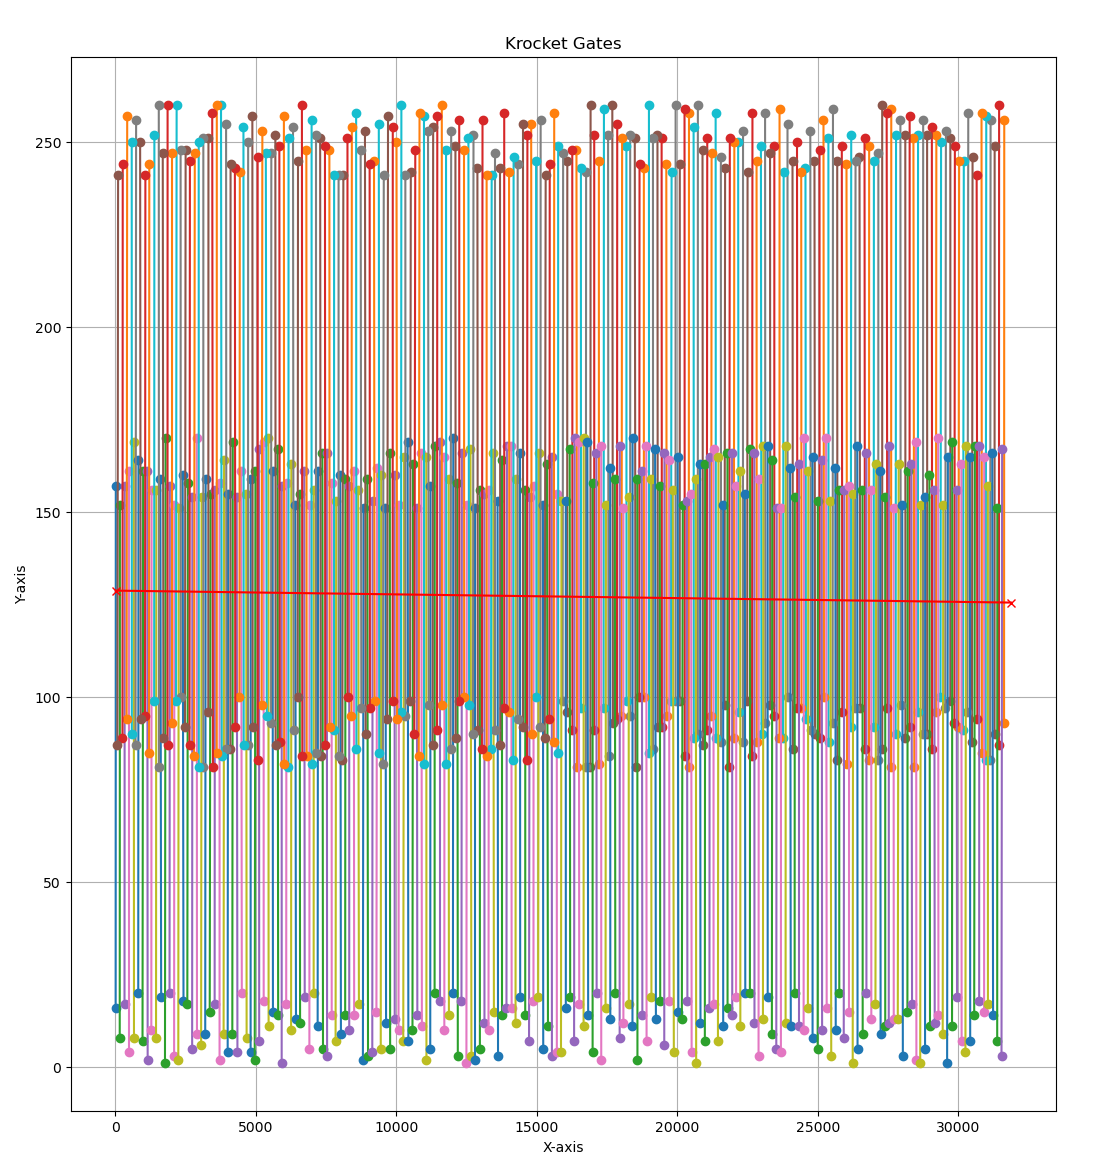
\includegraphics[scale=0.40]{krocket3.png}
  \newpage

  \item [4.] \textbf{krocket4.txt}
  \newline
  Es ist möglich mit einem Schlag alle Tore zu durchqueren.
  Der Schlag kann als Halbgerade mit dem Startpunkt: (6.14299999999999|182.9909999999977), die durch den 
  \newline Punkt (92.69300000000004|226.22499999999985) verläuft, beschrieben werden.
  \newline
  Normierter Richtungsvektor: (0.8945966401484378, 0.4468745365705309), bzw. Steigung der Halbgeraden: 0.4995262853841954
  \newline
  \newline
  Darstellung (python-skript)
  \newline
  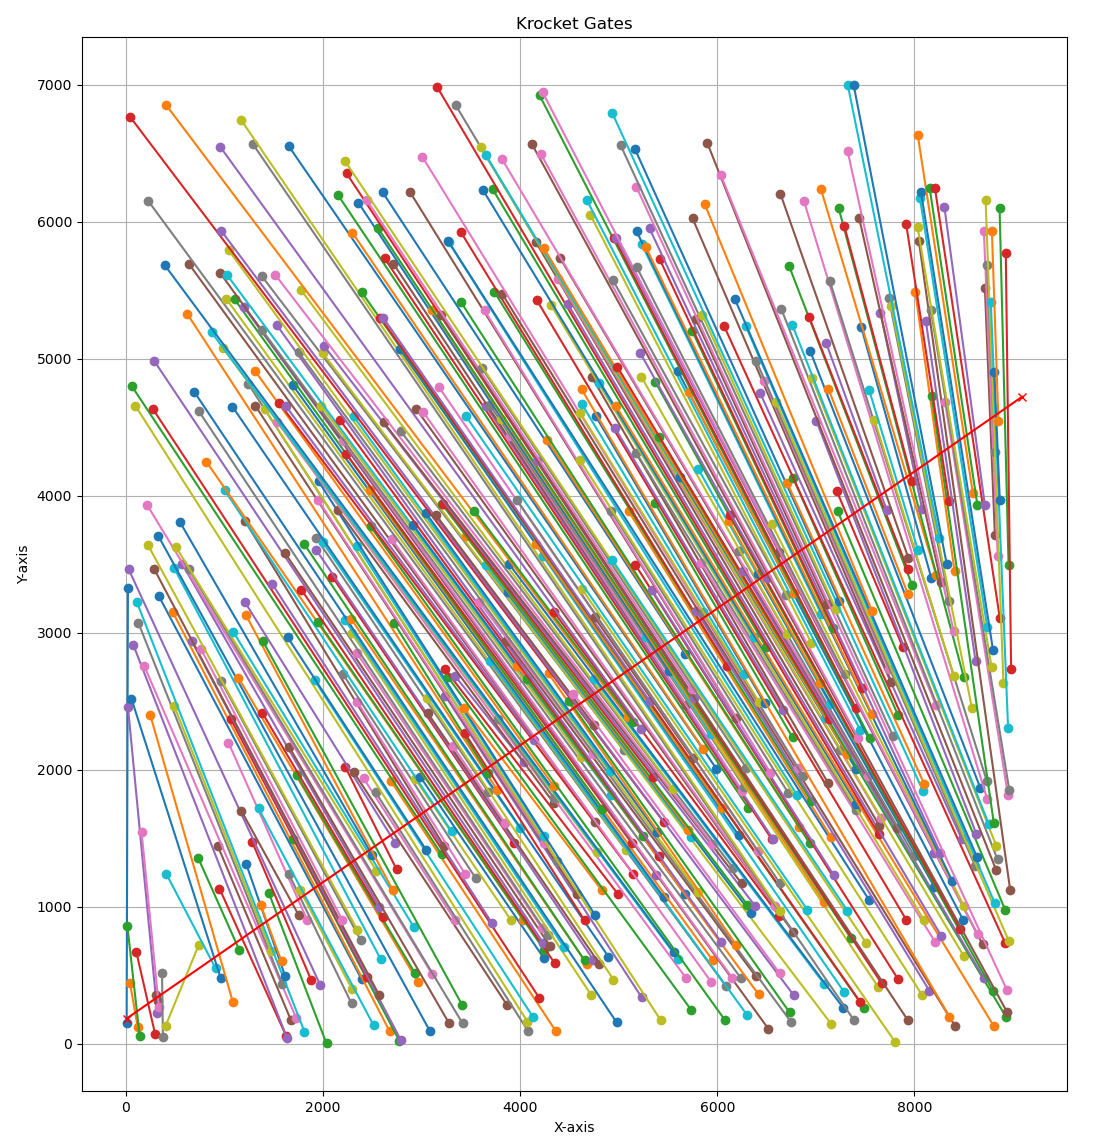
\includegraphics[scale=0.40]{krocket4.png}
  \newpage

  \item [5.] \textbf{krocket5.txt}
  \newline
  Es ist möglich mit einem Schlag alle Tore zu durchqueren.
  \newline
  Der Schlag kann als Halbgerade mit dem Startpunkt: (1314.4010000000007|14678.04), die durch den Punkt (3160.4020000000005|14215.655999999999) verläuft, beschrieben werden. 
  \newline
  Normierter Richtungsvektor: (0.9700331331504777, -0.24297267457528587), bzw. Steigung der Halbgeraden: -0.25047873755214756
  \newline
  \newline
  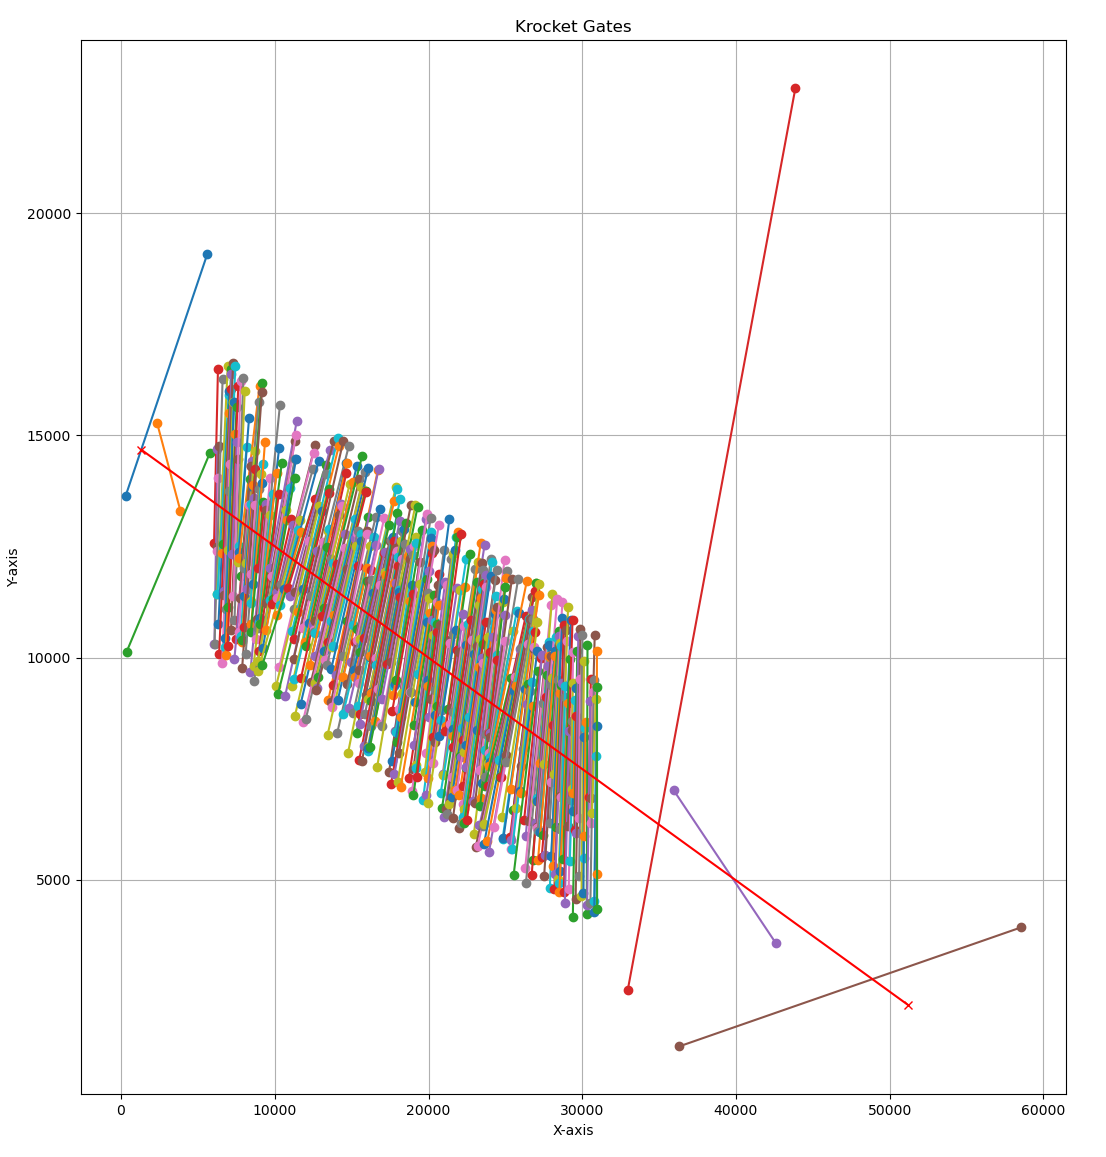
\includegraphics[scale=0.40]{krocket5.png}

\end{itemize}

\section{Quellcode}
\textbf{Finden einer Gerade, die alle Tore durchquert}
\begin{lstlisting}
/**
* Calculates a line that intersects all given gates
* The line intersects the starting point (placed on the first gate)
* Endpoint (direction of the line) for calculation of the line is on the second
* gate
* 
* @param gates    - List of gates the line has to intersect
* @param stepSize - Step size (0 to 1) percentage of the first gate's
*                 length, specifies how finely the starting points
*                 are iterated along the first gate
* @return Line - line that intersects all gates, null if no intersection
*/
public Line findRayIntersectAllGates(List<Gate> gates, double stepSize, double ballRadius) {
    Gate firstGate = gates.get(0);
    Gate secondGate = gates.get(1);

    // Iterate over positions on first gate in increments defined by step size
    // For every startpoint on the first gate, the loop is executed
    for (double stepStart = 0; stepStart <= 1; stepStart += stepSize) {
        // Create start point for the line on the first gate
        Point startPoint = new Point(
                firstGate.getStart().getX()
                        + stepStart * (firstGate.getEnd().getX() - firstGate.getStart().getX()),
                firstGate.getStart().getY()
                        + stepStart * (firstGate.getEnd().getY() - firstGate.getStart().getY()));

        // Iterate over positions on second gate in increments defined by step size
        for (double stepDir = 0; stepDir <= 1; stepDir += stepSize) {
            Point directionPoint = new Point(
                    secondGate.getStart().getX()
                            + stepDir * (secondGate.getEnd().getX() - secondGate.getStart().getX()),
                    secondGate.getStart().getY()
                            + stepDir * (secondGate.getEnd().getY() - secondGate.getStart().getY()));
            // Create line, that intersects startpoint and directionpoint
            Line gerade = new Line(startPoint, directionPoint);

            boolean intersectsAll = true;
            // Checks if line intersects all gates
            for (Gate gate : gates) {
                // Intersection between Segment and line
                Point intersectionSegmentGerade = calculateLineIntersectSegment(gerade, gate, ballRadius);
                // Does not intersect
                if (intersectionSegmentGerade == null) {
                    intersectsAll = false;
                    break;
                }
            }
            if (intersectsAll) {
                return gerade;
            }
        }
    }
    return null;
}
\end{lstlisting}

\textbf{Schnittpunkt einer Geraden mit einer Strecke}
\begin{lstlisting}
/**
* Calculates point of intersection of a line and a segment (krocket gate)
* 
* @param line - line to describe possible path of krocket ball
* @param gate - Krocketgate (segment)
* @return Point - Point of intersection; null if no intersection exists
*/
public Point calculateLineIntersectSegment(Line line, Gate gate, double ballRadius) {
    double lineStartX = line.getStart().getX();
    double lineStartY = line.getStart().getY();
    double dx = line.getDeltaX();
    double dy = line.getDeltaY();
    double gateStartX = gate.getStart().getX();
    double gateStartY = gate.getStart().getY();
    double gateEndX = gate.getEnd().getX();
    double gateEndY = gate.getEnd().getY();

    // More info in the documentation of this task

    // To calculate the intersection the equation of the line and gate have to be
    // equated
    // A system of linear equation can be set up for that
    // Then solve for unknown (u & t)
    // Which can be interpreted as a 2x2 matrix

    // Calculate determinant of equation system
    double denominator = dx * (gateEndY - gateStartY) - dy * (gateEndX - gateStartX);

    // If determinant is (almost) zero, the line and gate (segment) are parallel or
    // colinear
    // Therefore they cant have an intersection
    if (Math.abs(denominator) < 1e-10) {
        return null;
    }

    // Solve the system of equations
    // (I used gauss algorithm)
    double t = ((gateStartX - lineStartX) * (gateEndY - gateStartY)
            - (gateStartY - lineStartY) * (gateEndX - gateStartX)) / denominator;
    double u = ((gateStartX - lineStartX) * dy - (gateStartY - lineStartY) * dx) / denominator;

    // Check if the intersection point is outside of the gate segment 
    if (u < 0 || u > 1) {
        return null;
    }

    // Calculate the intersection point on the line
    Point intersectionPoint = line.getPointAt(t);

    // Check if the line intersects circle (collision boundary of start and endpoint
    // of gate)
    if (lineIntersectsCircle(line, gate.getStart(), ballRadius) ||
            lineIntersectsCircle(line, gate.getEnd(), ballRadius)) {
        return null; // Intersection invalid due to collision with gate endpoints
    }

    // Valid intersection point with enough space to gate endpoints
    return intersectionPoint;
}
\end{lstlisting}

\textbf{Schnittpunkte einer Gerade und einem Kreis}
\begin{lstlisting}
/**
* Check if a line intersects a circle
* 
* @param line         - line
* @param circleCenter - center of the circle as a Point
* @param radius       - radius of circle as double
* @return true if the line intersects the circle, else false
*/
private boolean lineIntersectsCircle(Line line, Point circleCenter, double radius) {
    double cx = circleCenter.getX();
    double cy = circleCenter.getY();
    double x1 = line.getStart().getX();
    double y1 = line.getStart().getY();
    double dx = line.getDeltaX();
    double dy = line.getDeltaY();

    // More info in the docs of this task
    // circle equation: (x - cx)^2 + (y - cy)^2=r^2
    // line equation: x = x1 + t * dx
    // &&
    // line equation: y = y1 + t * dy
    // Short: plug line equation into circle equation and solve for t
    double a = dx * dx + dy * dy;
    double b = 2 * (dx * (x1 - cx) + dy * (y1 - cy));
    double c = (x1 - cx) * (x1 - cx) + (y1 - cy) * (y1 - cy) - radius * radius;

    // Solve quadratic equation a*t^2 + b*t + c = 0 and just check discriminant
    // If discriminant < 0: no intersection
    // = 0: one intersection = line is a tangent
    // > 0: two intersections
    double discriminant = b * b - 4 * a * c;

    if (discriminant <= 0) {
        return false; // No real number
    } else {
        return true;
    }
}
\end{lstlisting}

\end{document}